Show that the only traveling "front" wave $u(x, t) = \phi (x - ct)$ with $\phi(-\infty) = 1$ and $\phi(+\infty) = 0$ 
which satisfies the PDE is

$$
u(x, t) = \left[ 1 + e^{\frac{1}{\sqrt{6}} x - \frac{5}{6} t } \right]^{-2}
$$

by deriving the ODE that $\phi$ must satisfy. Solve the resulting ODE numerically and, if possible, analytically.

\begin{solution}
    We begin with the observation that 



    We begin by defining $z = x - ct$ and observing that $u(x, t) = \phi(z)$ admits the following partial derivatives:

    \begin{align*}
        u_t &= \frac{\partial \phi}{\partial z} \frac{\partial z}{\partial t} = -c \phi_z, \\
        u_x &= \frac{\partial \phi}{\partial z} \frac{\partial z}{\partial x} = \phi_z, \\
        u_{xx} &= \frac{\partial }{\partial z} \frac{\partial z}{\partial x} \phi_z = \phi_{zz} \\
    \end{align*}

    so that Fisher's equation becomes the second-order ODE

    $$
    -c \phi_z = \phi_{zz} + \phi(1 - \phi)
    $$

    which is equivalent to the following system of ODEs:

    $$
        \begin{cases}
        \phi' = v \\
           v' = -c v - \phi(1 - \phi).
        \end{cases}
    $$

    We write our provided traveling front wave solution in terms of $z$ (with $c = \frac{5}{\sqrt{6}}$):

    $$
    u(x, t) = \left[ 1 + e^{\frac{1}{\sqrt{6}} \left(x - \frac{5}{\sqrt{6}} t \right) } \right]^{-2} 
            = \left[ 1 + e^{\frac{z}{\sqrt{6}}} \right]^{-2} 
            = \phi(z).
    $$

    Differentiating $\phi$ with respect to $z$ yields

    $$
    \phi'(z) = -\frac{2}{\sqrt{6}} e^{\frac{z}{\sqrt{6}}} \left[ 1 + e^{\frac{z}{\sqrt{6}}} \right]^{-3} 
    $$

    so that our initial condition are $\phi(0) = \frac{1}{4}$ and $v(0) = \phi'(0) = -\frac{1}{4 \sqrt{6}}$. With 
    $c = \frac{5}{\sqrt{6}}$, we can solve the system of ODEs numerically in $z$ using a fourth-order Runge-Kutta 
    method, which is implemented in \texttt{problem\_2i.m} and the output of which is shown in Figure 
    (\ref{fig:problem_2i}).

    \begin{figure}[h]
        \centering
        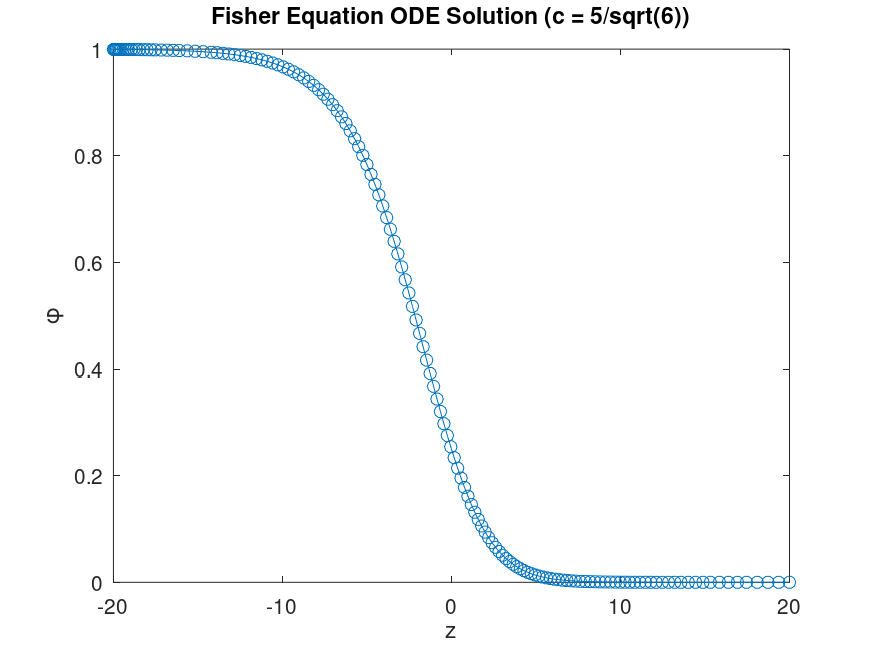
\includegraphics[width=0.8\textwidth]{problem_2i.png}
        \caption{Solution to Fisher ODE in $z = x - \frac{5}{\sqrt{6}} t$.}
        \label{fig:problem_2i}
    \end{figure}
    \ \\
\end{solution}